%%%%%%%%%%%%%%%%%%%%%%%%%%%%%%%%%%%%%
% Ch2 : Les liaisons interatomiques %
%%%%%%%%%%%%%%%%%%%%%%%%%%%%%%%%%%%%%

\chapter{Liaisons interatomiques}
\section{La liaison}
	Le but des liaisons est de remplir la couche de valence et de se rapprocher au plus de la configuration des gaz rares. L'existence de composés polyatomiques stables implique que les atomes soient capable de former des agrégats dont \textbf{l'énergie est plus faible que s'ils étaient isolés}. Les types de liaison dépendent de l'agencement des électrons de valence et sont au nombre de 4 : \\

\begin{itemize}
	\item[•] la liaison ionique
	\item[•] la liaison covalente
	\item[•] la liaison métallique
	\item[•] les liaisons secondaires hydrogène et de Vander Waals. \\
\end{itemize}
	
Les 3 premières sont des liaisons fortes alors que les dernières sont plus faibles. Soulignons que, le plus souvent, la liaison des atomes dans un solide présente un caractère mixte associant des contributions simultanées de plusieurs types liaisons chimiques.

\section{Types de liaisons}
	\section{La liaison ionique, opportunisme individualiste}
		Liaison qui implique le transfert d'électrons depuis un atome vers un autre. Type de liaison qui détermine la cohésion des solides constitués de l'association d'atomes possédant des affinités électronique très différentes. Prenons l'exemple du sel de cuisine $NaCl$ et regardons ce qui se passe d'un point de vue énergétique. Tout d'abord, l'énergie de première ionisation de $Na$ et l'affinité électronique (énergie libéré lorsqu'un électron est capté) de $Cl$ sont
		\begin{equation}
			E_{ion}\, Na= 5.14 \, eV \qquad et \qquad \mbox{Aff.élec } Cl = 4.02 \, eV 
		\end{equation}	 
		ce qui veut dire qu'il faut $U_i = 1.12\, eV$ pour séparer $NaCl$ en $Na^++Cl^-$. Il faut encore tenir compte de la force électrostatique $F$ entre les deux ions de charges différentes. Quand un ion se rapproche depuis l'infini, 
		\begin{equation}
			U_a = \int _\infty ^r F_{attr} \, dr= \int _\infty ^r \frac{q^2}{4\pi \epsilon _0 r^2} \, dr = -\frac{q^2}{4\pi \epsilon _0 r}
		\end{equation}
		Le signe négatif de cette énergie traduit le fait que les ions ont tendance à se rapprocher. Cependant, à très petite distance, les cortèges électroniques commencent à se superposer et une forte répulsion apparaît selon 
		\begin{equation}
			U_r = \frac{B}{r^n}
		\end{equation}
		\begin{wrapfigure}[5]{l}{6.5cm}
		\vspace{-14mm}
		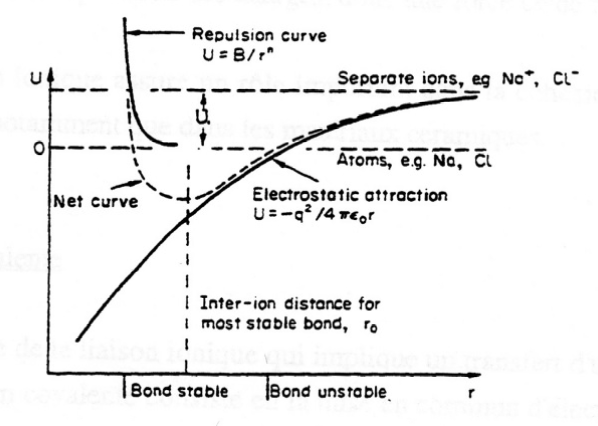
\includegraphics[scale=0.6]{ch2/1}
		\end{wrapfigure}
		La somme de toutes ces contributions donne la courbe d'énergie potentielle suivante. La distance d'équilibre $r_0$ correspond au minimum. \\
	En conclusion, cette liaison est \textbf{forte}, de nature \textbf{électrostatique} et \textbf{non-directionnelle}. \\\\

	\subsection{La liaison covalente, communisme à courte distance}
		Cette liaison consiste en la mise en commun d'électrons par deux atomes voisins. Dans la \textbf{covalente pure}, deux atomes identiques combinent leurs orbitales incomplètes afin de gagner les électrons manquants. \\
		Seules les orbitales $s$ ont une distribution spatiale \textbf{isotrope}, les autres sont \textbf{extrêmement anisotropes} entraînant une \textbf{directionnalité très marquée} à cause de la superposition partielle d'orbitales qui se fait grâce à l'hybridation. Cette liaison est de loin le type le plus fort. 
	
	\subsection{La liaison métallique, communisme à grande distance}
		\begin{wrapfigure}[5]{r}{2cm}
		\vspace{-5mm}
		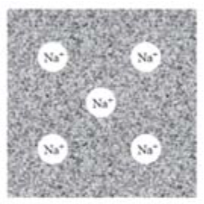
\includegraphics[scale=0.6]{ch2/2}
		\end{wrapfigure}
		Il s'agit d'une mise en commun d'électrons entre tous les atomes d'un solide. Les électrons périphériques sur les orbitales $s$ et $p$ sont faiblement liés et, lorsque les atomes se condensent, n'appartiennent plus à une orbitale localisée autour d'un atome. \\
		Pour représenter ça, on peut imaginer un empilement d'ions métalliques entouré par un \textbf{gaz d'électrons} constitué par la mise en communs des électrons les plus périphériques. Le déplacement des atomes depuis leur position d'équilibre est facile puisque le nuage peut se réorganiser pour contrer le déséquilibre de charge. \\
		Cette liaison est d'une force plus faible que les autres et est non-directionnelle puisqu'elle résulte de forces électrostatiques entre des ions et un gaz d'électrons. Le caractère métallique augmente à mesure que le nombre d'électrons diminue sur $s$ et $p$ et que l'attraction de ceux-ci par le noyau diminue (bas gauche dans le tableau périodique).
		
	\subsection{Les liaisons secondaires}
		\subsubsection{Van der Waals}  
			\begin{wrapfigure}[6]{l}{6.5cm}
			\vspace{-7mm}
			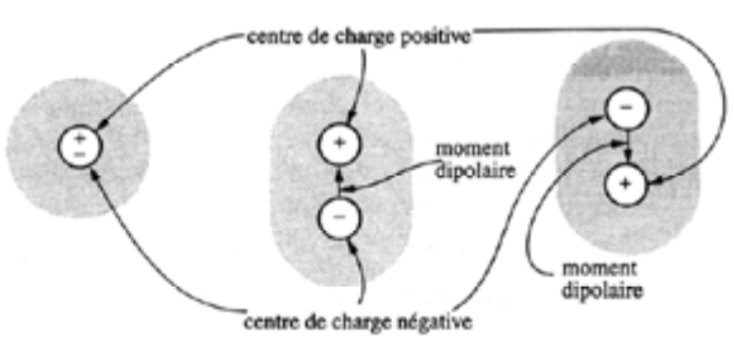
\includegraphics[scale=0.5]{ch2/3}
			\end{wrapfigure}
			Ici, la charge électronique est en perpétuel mouvement traduisant une répartition de la charge non symétrique. Les atomes possèdent donc un \textbf{moment dipolaire instantané} non nul induisant une modification dans la répartition des charges des cortèges électroniques des voisins, conduisant ainsi à un autre dipôle instantané. \\
			Leur orientation est telle qu'ils s'attirent mutuellement $\rightarrow$ liaison de Vander Waals. Elle est faible et parfaitement non-directionnelle.
			
		\subsubsection{Liaison hydrogène}
			Quand l'hydrogène forme une liaison covalente polarisée avec un atome électronégatif, c'est lui qui est le pôle positif. Il devient alors capable d'interagir avec les électrons périphériques des atomes électronégatifs des molécules voisines. \\
			La force de cette liaison est $\approx 1/10$ fois la force de la liaison covalente et joue. Elle joue un rôle important dans la cohésion des molécules d'eau.
			
\section{Les matériaux}
	\subsection{Les classes}
		Les liaisons chimiques dictent les propriétés d'un solide. On classe les matériaux en 4 classes :
	
		\begin{enumerate}
			\item \textbf{Les céramiques :} liaisons covalente et/ou ionique
			\item \textbf{Les métaux :} liaison métallique
			\item \textbf{Les polymères :} liaisons covalente \textbf{et} secondaire
			\item \textbf{Les composites :} mélange de 2 types de matériaux (ex : polymères renforcés par des fibres céramiques)
		\end{enumerate}	 
	
	\subsection{Implications des liaisons}
		\subsubsection{La liaison ionique}
			\begin{itemize}
				\item[•] Haut point de fusion dû à l'énergie de liaison élevée
				\item[•] Faible conductivité thermique et électrique due à l'indisponibilité d'électrons libres
				\item[•] Pas d'interaction avec les ondes électromagnétiques (transparence) dû à la même chose
				\item[•] Les cristaux sont peu malléables car si les plans cristallographique glissent, les charges de même signe sont face à face
			\end{itemize}					
			
		\subsubsection{La liaison covalente}
			\begin{itemize}
				\item[•] Haut point de fusion dû à l'énergie de liaison élevée
				\item[•] Faible conductivité thermique et électrique due à l'indisponibilité d'électrons libres. Semi-conductivité à haute température
				\item[•] Pas d'interaction avec les ondes électromagnétiques (transparence) dû à la même chose
				\item[•] Matériaux durs et cassant en raison des liaisons très fortes
			\end{itemize}		
		\subsubsection{La liaison métallique}
			\begin{itemize}
				\item[•] Excellente conductivité puisque les électrons ne sont plus liés à des atomes en particulier
				\item[•] Les électrons libre rendent les métaux opaques et réfléchissants
				\item[•] Maléable, doux et ductile du fait que les ions positifs ne sont pas directement lié
			\end{itemize}
			
		\subsubsection{La liaison de Vander Waals}
			\begin{itemize}			
			\item[•] Solides compressibles, mous et faibles propriétés mécaniques
			\item[•] Point de fusion très bas
			\item[•] Isolant électrique et mauvais conducteurs thermiques 
			\item[•] Participe à la cohésion de solides à liaison mixte : entre les atomes d'une même chaîne $\rightarrow$ covalente et entre les chaînes $\rightarrow$ secondaires
			\end{itemize}